\documentclass[12pt]{article}

\usepackage[backend=biber,style=mla]{biblatex}
\usepackage[margin=1in]{geometry}
\usepackage[utf8]{inputenc}
\usepackage{multicol}
\usepackage{setspace}
\usepackage{amsmath}
\usepackage{amssymb}
\usepackage{mathtools}
\usepackage{esint}
\usepackage{titlesec}
\usepackage{graphicx}
\usepackage{wrapfig}
\usepackage{blindtext}
\usepackage{fancyhdr}

\addbibresource{/home/krttd/Documents/UAH.bib}

\pagestyle{fancy}
\lhead{}
\chead{}
\cfoot{}
\rhead{Dodson \thepage}

\renewcommand*{\bibfont}{\normalsize}

\titleformat{\section}
{\large}{}{0em}{}[\titlerule]


\begin{document}

\begin{center}\LARGE
Writing Software Design Documentation
\end{center}

\begin{center}\large
	Mitchell T. Dodson; Eh 301; March 24, 2020
\end{center}

\begin{multicols}{2}

	\section{Purpose --}

	Software design documentation is generally tailored towards professional software customers or people who will utilize or modify a body of software in the future. Effective software design documentation aims to make the production, transition, and maintenance of a body of software as effective and efficient as possible by clearly outlining the software's design and intended usage.

	\section{Features -- }

	Effective software documentation includes an abstract description of the purpose of the body of software as a whole, a logical breakdown of discrete software modules with descriptions of each's role in the program, as well as unambiguous description of each module's arguments and outputs. Presenting the neccesary information with diagrams such as flow charts (example below) is often the most effective way to convey the exchange of information among modules in a program.

	\vspace{1em}
	\begin{center}
		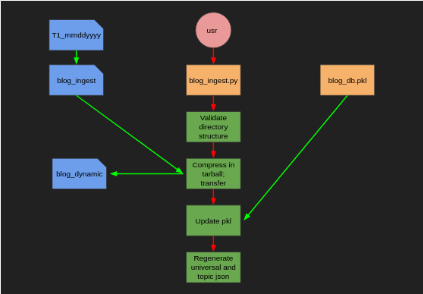
\includegraphics[width=.9\linewidth]{./figures/flowchart.png}

		\vspace{.4em}
		Flow Chart Example
	\end{center}

	\columnbreak

	\section{Keep in mind -- }

	\begin{itemize}
		\item{Many readers will want to skim documentation to find specific information; make sections clear and distinct}
		\item{Fine details of how software is implemented are unneccesary; focus on arguments and return standards for abstract components of the program}
		\item{Include examples that utilize important features of the softwrae and demonstrate how to apply the software to common use cases}
		\item{Software design documentation should be considered an elaboration on inline documentation; don't hesitate to repeat information found elsewhere.}
		\item{Do your best to anticipate and offer solutions to issues that readers may encounter while applying or modifying the program}
	\end{itemize}

	\section{Examples --}

	\texttt{man} pages - Manual ('man') pages are a form of documentation commonly shipped with command-line utilities. Though intended for end-users, man pages typically contain ample API documentation for programmers who want to incorporate the program into other software. the manual for \texttt{ffmpeg} is especially well-written. To access, simply pass

	\begin{center}
		\texttt{\$ man <software\_name>}
	\end{center}

	\noindent
	into any console on your machine, replacing $<$software\_name$>$ with the actual title of an installed program

\end{multicols}

\printbibliography
\end{document}
